\documentclass[xcolor=x11names]{beamer}
%%%%%%%%%%%%%%%%%%%%%%%%%%%%%%%%%%%%%%%%%%%%%%%%%%%%%%%%%%%%
%%  This Beamer template was created by Cameron Bracken.
%%  Anyone can freely use or modify it for any purpose
%%  without attribution.
%%
%%  Last Modified by C. Bracken: January 9, 2009
%%
%%  The preamble, and maybe some modification of the Cameron Bracken's template is due to Attila Molnár.
%%
%%

%% General document
\usepackage[utf8]{inputenc}
\usepackage[T1]{fontenc}
\usepackage{graphicx}
\usepackage{tikz}
\usetikzlibrary{decorations.fractals}
\usetikzlibrary{decorations.text}
\usepgflibrary{arrows}
\usetikzlibrary{fadings}
\usetikzlibrary[decorations.pathmorphing]
\tikzfading[name=fade inside, inner color=transparent!70, outer color=transparent!70]
\usetikzlibrary{calc}
\usetikzlibrary{intersections}
\usetikzlibrary{shapes}
\usetikzlibrary{patterns}
\usefonttheme{serif}
\usepackage{amssymb} 			
\usepackage{amsmath}
\usepackage{ifthen}
\usepackage[normalem]{ulem}
\usepackage{mathrsfs}

%%%%%%%%%%%%%%%%%%%%%%%%%%%%%%%%%%%%%%%%%%%%%%%%%%%%%%%%%%%%%%%%%%%%%%%%%%%%%%%%%%%%
%% Beamer Layout %%%%%%%%%%%%%%%%%%%%%%%%%%%%%%%%%%
\useoutertheme[subsection=false,shadow]{miniframes}
\useinnertheme{default}
\usefonttheme{serif}
%\usepackage{txfonts} %Hook for strict implication!
\DeclareSymbolFont{symbolsC}{U}{txsyc}{m}{n}
\DeclareMathSymbol{\strictif}{\mathrel}{symbolsC}{74}
\DeclareMathSymbol{\boxright}{\mathrel}{symbolsC}{128}
\usepackage{palatino}
%\usepackage[uppercase=upright,charter]{mathdesign}

\setbeamerfont{title like}{shape=\scshape}
\setbeamerfont{frametitle}{shape=\scshape}


\setbeamercolor*{lower separation line head}{bg=white!40!DeepSkyBlue3}
\setbeamercolor*{normal text}{fg=black,bg=white}
\setbeamercolor*{alerted text}{fg=red}
\setbeamercolor*{example text}{fg=black}
\setbeamercolor*{structure}{fg=black}

\setbeamercolor*{palette tertiary}{fg=black,bg=white!90!DeepSkyBlue3}
\setbeamercolor*{palette quaternary}{fg=black,bg=black!10}

%\setbeamercolor{block body alerted}{bg=normal text.bg!90!DeepSkyBlue4}
\setbeamercolor{block body}{bg=normal text.bg!95!DeepSkyBlue3}
%\setbeamercolor{block body example}{bg=normal text.bg!90!DeepSkyBlue4}
%\setbeamercolor{block title alerted}{use={normal text,alerted text},fg=alerted text.fg!75!normal text.fg,bg=normal text.bg!90!DeepSkyBlue4}
\setbeamercolor{block title}{bg=normal text.bg!70!DeepSkyBlue3}
%\setbeamercolor{block title example}{use={normal text,example text},fg=example text.fg!75!normal text.fg,bg=normal text.bg!75!DeepSkyBlue4}

\setbeamertemplate{blocks}[rounded][shadow=true]
%\setbeamertemplate{background canvas}[vertical shading][bottom=white,top=structure.fg!25]
%\setbeamertemplate{sidebar canvas left}[horizontal shading][left=white!40!black,right=black]
\setbeamertemplate{itemize items}[circle]
\setbeamercolor*{itemize item}{fg=DeepSkyBlue3}
\setbeamercolor*{itemize subitem}{fg=DeepSkyBlue3}
\setbeamercolor*{itemize subsubitem}{fg=DeepSkyBlue3}
\setbeamertemplate{enumerate items}[circle]
%\setbeamercolor{item projected}{bg=DeepSkyBlue3,fg=black}
\setbeamercolor{item projected}{bg=white,fg=DeepSkyBlue3}
\setbeamercolor*{enumerate item}{fg=DeepSkyBlue3}
\setbeamercolor*{enumerate subitem}{fg=DeepSkyBlue3}
\setbeamercolor*{enumerate subsubitem}{fg=DeepSkyBlue3}

%%%%%%%%%%%%%%%%%%%%%%%%%%%%%%%%%%%%%%%%%%%%%%%%%%


%%%%%%%%%%%%%%%%%%%%%%%%%%%%%%%%%%%%%%%%%%%%%%%%%%%%%%%%%%%%%%%%%%%%%%%%%%%%%%%%%%%%

\newenvironment{defi}[1][]{\begin{block}{\footnotesize \textsc{Definition} \ifthenelse{\equal{#1}{}}{}{\, (#1)}}}{\end{block}}
\newenvironment{prop}[1][]{\begin{block}{\footnotesize \textsc{Proposition} \ifthenelse{\equal{#1}{}}{}{\, (\textsc{#1})}}}{\end{block}}
\newenvironment{lemm}[1][]{\begin{block}{\footnotesize \textsc{Lemma} \ifthenelse{\equal{#1}{}}{}{\, (\textsc{#1})}}}{\end{block}}
\newenvironment{idea}[1][]{\begin{block}{\footnotesize \textsc{Idea} \ifthenelse{\equal{#1}{}}{}{\, (\textsc{#1})}}}{\end{block}}
\newenvironment{rema}[1][]{\begin{block}{\footnotesize \textsc{Remark} \ifthenelse{\equal{#1}{}}{}{\, (\textsc{#1})}}}{\end{block}}
\newenvironment{coro}[1][]{\begin{block}{\footnotesize \textsc{Corollary} \ifthenelse{\equal{#1}{}}{}{\, (\textsc{#1})}}}{\end{block}}
\newenvironment{tete}[1][]{\begin{block}{\footnotesize \textsc{Theorem} \ifthenelse{\equal{#1}{}}{}{\, (\textsc{#1})}}}{\end{block}}
\newenvironment{claim}[1][]{\begin{block}{Claim \ifthenelse{\equal{#1}{}}{}{\, (\textsc{#1})}}}{\end{block}}
%\newenvironment{lemma}[1][]{\begin{block}{Lemma \ifthenelse{\equal{#1}{}}{}{\, (\textsc{#1})}}}{\end{block}}
\newenvironment{question}[1][]{\begin{block}{Question \ifthenelse{\equal{#1}{}}{}{\, (\textsc{#1})}}}{\end{block}}
\newenvironment{rem}[1][]{\begin{block}{Remark \ifthenelse{\equal{#1}{}}{}{\, (\textsc{#1})}}}{\end{block}}
\newenvironment{homework}[1][]{\begin{block}{Homework \ifthenelse{\equal{#1}{}}{}{\, (\textsc{#1})}}}{\end{block}}
\newenvironment{proo}[1][]{\begin{block}{\footnotesize \textsc{Proof} \ifthenelse{\equal{#1}{}}{}{\, (\textsc{#1})}}}{\end{block}}

%%%%%%%%%%%%%%%%%%%%%
%% To evade unnecessary circles, mainly for \cimdia
%%%%%%%%%%%%%%%%%%%%%

\makeatletter
\let\beamer@writeslidentry@miniframeson=\beamer@writeslidentry
\def\beamer@writeslidentry@miniframesoff{%
  \expandafter\beamer@ifempty\expandafter{\beamer@framestartpage}{}% does not happen normally
  {%else
    % removed \addtocontents commands
    \clearpage\beamer@notesactions%
  }
}
\newcommand*{\miniframeson}{\let\beamer@writeslidentry=\beamer@writeslidentry@miniframeson}
\newcommand*{\miniframesoff}{\let\beamer@writeslidentry=\beamer@writeslidentry@miniframesoff}
\makeatother

%%%%%%%%%%%%%%%%%%%%%%%%%%%%%
%%%%%%%%%%%%% END %%%%%%%%%%%
%%%%%%%%%%%%%%%%%%%%%%%%%%%%%


%%%% Formatting Commands

\newcommand{\cimdia}[1] {\miniframesoff \begin{frame}\begin{center}\huge \begin{tabular}{c}#1\end{tabular}\end{center}\end{frame}\miniframeson}
\newcommand{\szakasz}[2][]{\section{#1}\subsection{}\cimdia{#2}}
\newcommand{\bluebullet}{\textcolor{DeepSkyBlue3}{\quad $\bullet$} \,\,}

\newenvironment{frame*}[1][]{\miniframesoff \begin{frame} #1}{\end{frame}\miniframeson}

  % for admissible intersections
  \newcommand{\bigsqcap}{\rotatebox[origin=c]{180}{$\bigsqcup$}}

  % Intelligent curves for tikz:
  % Use it in this way: \gorbe{elejenev}{vegenev}{elejeszog}{elejelendulet}{vegeszog}{vegelendulet};
  \newcommand{\gorbe}[6]{\draw (#1).. controls ([shift=(#3: #4 cm)]#1) and ([shift=(#5: #6 cm)]#2) .. (#2);}
  \newcommand{\gorbefelirattal}[8]{\draw (#1).. controls ([shift=(#3: #4 cm)]#1) and ([shift=(#5: #6 cm)]#2) .. (#2) node[#8] {#7};}

\newcommand{\pipa}{%
\begin{tikzpicture}[green!50!black, thick, scale=.1]
\gorbe{0,1}{2,2}{-80}{1}{225}{.7}
\end{tikzpicture}}

\newcommand{\ellentmondas}
		{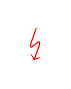
\begin{tikzpicture}[scale=0.2]
			\draw[rounded corners=3pt, rotate=10, red,
					->] (0.75,2)--(0,0.66)--(1,1.33)--(0.25,0);
		\end{tikzpicture}}
\newcommand{\indirektfelteves}
		{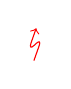
\begin{tikzpicture}[scale=0.2]
			\draw[rounded corners=3pt, rotate=10, red,
					<-] (0.75,2)--(0,0.66)--(1,1.33)--(0.25,0);
		\end{tikzpicture}}

\newcommand{\pecset}[2]{\begin{tikzpicture}[remember picture,overlay]
\node [ draw=red,
        rectangle,
        rounded corners=5mm,
        inner sep=1mm,
        ultra thick,
        fill=white,
        fill opacity=.8,
        rotate=30,
        scale=#1,
        text opacity=0.7]
        at (current page.center)
        {#2};
\end{tikzpicture}}

%\felirat{inner sep}{rounded corners}{scale}{x}{y}{text}
\newcommand{\felirat}[7][]{\begin{tikzpicture}[remember picture,overlay]
\node [draw=DeepSkyBlue3, rectangle, rounded corners=#3 mm, inner sep=#2mm, ultra thick, fill=white, fill opacity=.8, scale=#4, text opacity=1,#1]
at ([xshift=#5 cm, yshift=#6 cm]current page.center) {#7};
\end{tikzpicture}}

\newcommand{\hazi}[6]{\begin{tikzpicture}[remember picture,overlay]
\node [ draw=Coral1,
        rectangle,
        rounded corners=#2 mm,
        inner sep=#1mm,
        ultra thick,
        fill=white,
        fill opacity=.8,
        rotate=0,
        scale=#3,
        text opacity=1]
        at ([xshift=#4 cm, yshift=#5 cm]current page.center)
        {#6};
\end{tikzpicture}}


% Emphasizing:
\definecolor{barna}{rgb}{0.5,0.2,0.1}
\newcommand{\bemph}[1] {{\color{DeepSkyBlue3}{#1}}}
\newcommand{\kemph}[1] {{\color{blue}{#1}}}
\newcommand{\cemph}[1]{\textcolor{red}{#1}}
\newcommand{\zemph}[1] {{\color{Green2}{#1}}}
\newcommand{\yemph}[1] {{\color{Orange1}{#1}}}
\renewcommand{\emph}[1]{\textbf{#1}}

\newcommand{\FD}{\mathbf F}
\newcommand{\FB}{\mathbf G}
\newcommand{\PD}{\mathbf P}
\newcommand{\PB}{\mathbf H}

\newcommand{\FDDot}{\underline{\mathbf F}}
\newcommand{\FBDot}{\underline{\mathbf G}}
\newcommand{\PDDot}{\underline{\mathbf P}}
\newcommand{\PBDot}{\underline{\mathbf H}}


% i dont know whats this
\newcommand{\matbuborek}[1]{%
\begin{tikzpicture}
\node[draw=black, rounded corners=2pt, rectangle, inner sep=1mm] at (0,0){$#1$};
\end{tikzpicture}}


\newcommand{\dzsa}[1]{\textsc{\underline{#1}}:}

% modal operators:
 \newcommand{\diamondmeret}{.18}
 \newcommand{\boxmeret}{4*\diamondmeret/5}


 \newcommand{\mland} [1][.1]{\hspace{#1cm}\textup{and}\hspace{#1cm}}
 \newcommand{\mlthen}[1][.1]{\hspace{#1cm}\Rightarrow\hspace{#1cm}}
 \newcommand{\mlnot} [1][.1]{\hspace{#1cm}\textup{not }}
 \newcommand{\mlor}  [1][.1]{\hspace{#1cm}\textup{or}\hspace{#1cm}}
 \newcommand{\mliff} [1][.1]{\hspace{#1cm}\mliff\hspace{#1cm}}
 \newcommand{\vonal} [1][.2]{\hspace{#1cm} | \hspace{#1cm}}
 \newcommand{\mlwhere} [1][.2]{\hspace{#1cm}\textup{where}\hspace{#1cm}}
 \newcommand{\lrule}[3][c]{\begin{array}{#1} #2  \\  \hline #3 \end{array}}
 \newcommand{\dlrule}[3][c]{\begin{array}{#1} #2  \\  \hline\hline #3 \end{array}}
 \newcommand{\dual}{\delta}
\newcommand{\Dajmond}{\lozenge}
\newcommand{\Boksz}{\square}
\newcommand{\felDajmond}{\blacklozenge}
\newcommand{\felBoksz}{\blacksquare}
\newcommand{\felle}	
	{\,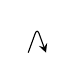
\begin{tikzpicture}
		\pgfmathsetmacro{\szog}{70}
		\pgfmathsetmacro{\hossz}{0.33}
	\draw[->,>=stealth,rounded corners=2pt] (0,0)	--(\szog:\hossz cm)
								--([shift=(-\szog :\hossz cm)]\szog:\hossz cm);	
	\end{tikzpicture}\,}
\newcommand{\lefel}
	{\, 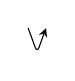
\begin{tikzpicture}
		\pgfmathsetmacro{\szog}{70}
		\pgfmathsetmacro{\hossz}{0.33}
		\draw[->,>=stealth,rounded corners=2pt] (0,0)	--(-\szog:\hossz cm)
								--([shift=(\szog :\hossz cm)]-\szog:\hossz cm);
	\end{tikzpicture}\, }
\newcommand{\enn}
{\mathbf{N}}
\newcommand{\nne}
{\reflectbox{$\mathbf{N}$}}

\newcommand{\mono}{\rightarrowtail}
\newcommand{\epi}{\twoheadrightarrow}
\newcommand{\iso}{\rightarrowtail \!\!\!\!\! \rightarrow}

 \newcommand{\defegy}[1][.1]{\hspace{#1cm}\overset{\textup{\tiny def}}{=}\hspace{#1cm}}
 \newcommand{\defpont}[1][.1]{\hspace{#1cm}\overset{\textup{\tiny def}}{:}\hspace{#1cm}}
 \newcommand{\defekv}[1][.1]{\hspace{#1cm}\overset{\textup{\tiny def}}{ \Leftrightarrow }\hspace{#1cm}}
 \newcommand{\lthen}{\rightarrow}
 \newcommand{\liff}{\leftrightarrow}
 \newcommand{\lminus}{-}
 \newcommand{\lsup}{\mbox{$\mathop{\sim}$}}
 \newcommand{\colnot}{\mbox{$\mathop{\sim}$}}
 \newcommand{\forallin}[2]{(\forall #1 \in #2)}
 \newcommand{\existsin}[2]{(\exists #1 \in #2)}
 \newcommand{\nexistsin}[2]{(\nexists #1 \in #2)}
 \newcommand{\forallp}[1]{(\forall #1)}
 \newcommand{\existsp}[1]{(\exists #1)}
 \newcommand{\forallR}[2]{(\forall #1 \reflectbox{$R$} #2)}
 \newcommand{\existsR}[2]{(\exists #1 \reflectbox{$R$} #2)}
\newcommand{\magyarazat}[2]{\overset{\substack{\textup{#2}\\ \downarrow}}{#1}}


\newcommand{\bintension}[2][]{{{[}\!{[}} {#2}{{]}\!{]}}^{\mathcal{#1}}}
\newcommand{\wintension}[3][]{{[}\hspace{-.46mm}{[} {#3}{]}\hspace{-.46mm}{]}^{\mathfrak{#1}}_{#2}}
\newcommand{\canintension}[2][]{{[}\hspace{-.46mm}{[} {#2}{]}\hspace{-.46mm}{]}_{\mathrm{#1}}}
\newcommand{\jelentes}[2]{{{[}\!{[}} {#1}{{]}\!{]}}^{{#2}}}
\newcommand{\intension}[2][]{{[}\hspace{-.46mm}{[} {#2}{]}\hspace{-.46mm}{]}^{\mathfrak{#1}}}
\newcommand{\Kintension}[2][]{|\!| {#2} |\!|^{\mathcal{#1}}}
\newcommand{\theory}[2][]{\mathrm{th}_{\mathfrak{#1}}(#2)}
\newcommand{\seenby}{\reflectbox R}
\newcommand{\derives}[1][]{\vdash_{\mathrm{#1}}}
\newcommand{\ugyanaz}[1]{\mathrel{\overset{#1}{\equiv}}}


\newcommand{\harmasosztas}[6]{

\begin{minipage}{#1\textwidth}%
#4%
\end{minipage}%
\begin{minipage}{#2\textwidth}%
#5%
\end{minipage}%
\begin{minipage}{#3\textwidth}%
#6%
\end{minipage}

}


\newcommand{\felkor}[8]{%
\begin{scope}[draw=#5,very thick,fill opacity=.15,draw opacity=.5,text opacity=1]
\draw[fill=#5]
([shift=(#3:#2)]#1) arc (#3:180+#3:#2) -- cycle;
\node at ([shift=(#7*180+#3:#2),shift=(-#7*90+135+#3:0.5*#6)]#1){#8};
\clip ([shift=(#3:#2)]#1) arc (#3:180+#3:#2);
 \draw[fill=#5] ([shift=(#7*180+#3:#2)]#1) circle (#6);
\end{scope}
}
\newcommand{\felkorvonal}[2]{
\draw[rounded corners=0] (180+#1:.25*#2 cm) arc (180+#1:360+#1:.25*#2 cm)--cycle;
}


\newcommand{\BoxTemplate}[1]{{#1} \mathop{\Box\hspace{-1.35ex} \raisebox{.5ex}{\scalebox{.5}{$\lthen$}}}}
\newcommand{\DiamondTemplate}[1]{#1\hspace{-.2ex} \mathop{\Diamond\hspace{-1.35ex} \raisebox{.4ex}{\scalebox{.5}{$\land$}}}\,}

%%%%%%%%%%%%%%%%%%%%%%%%%%%%%%%%%%%%%%%%%%%%%%%%%%%%%%
\newenvironment{tomb}[2][.1]{\arraycolsep=#1cm\begin{array}{#2}}{\end{array}}
\beamertemplatenavigationsymbolsempty


\author{Attila Moln\'ar}
\date{2014. March 21.}
\title{Axiomatization of Kripkean FOML}
\institute{ELTE}
\begin{document}
\footnotesize


\begin{frame}
\centering
\textsc{\Large Temporal Logic \\[1em] Introduction}

\bigskip

{ \small Attila Moln\'ar

    \textit{E\"otv\"os Lor\'and University}}

 \begin{figure}

\includegraphics[scale=.3]{elte_cimer.png}
 \end{figure}

	\today
\end{frame}

\szakasz[Intro]{Introduction}

\begin{frame}%[t]
	\frametitle{McTaggart 1908}
\footnotesize
There are two ways of speaking about time:
\begin{itemize}
\item[A-series:] with singular predicates: ``\dots is past'', ``\dots is present'', ``\dots is future'' (maybe builted in tenses ``was'', ``is'', ``will''). Note that the truth of these sentences depends on the time of the utterance. \emph{Local} perspective.
    \[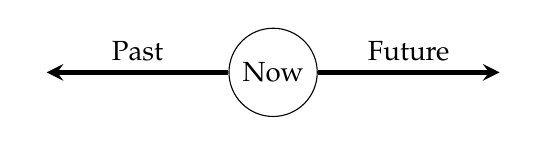
\begin{tikzpicture}[>=stealth]
    \node(now)[circle, draw=black] at (0,0) {Now};
    \node(future) at (3,0) {};
    \node(past) at (-3,0) {};
    \draw[->, ultra thick] (now)--(future) node[midway, above]{Future};
    \draw[->, ultra thick] (now)--(past) node[midway, above]{Past};
    \end{tikzpicture}\]
\item[B-series:] with ordering relations: ``\dots comes before \dots'', ``\dots comes after \dots''. The truth of these sentences does not depend on the time of the utterance. \emph{Global} perspective.
    \[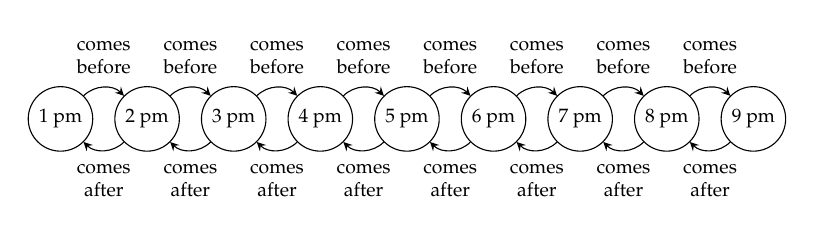
\begin{tikzpicture}[>=stealth]
    \foreach \i in {1, 2, ..., 9}
    {\node[scale=.7](\i)[circle, draw=black] at (1.1*\i,0) {\i~pm};}
    \foreach \i in {1, 2, ..., 8}
    {\pgfmathtruncatemacro{\j}{\i + 1}
    \draw[->](\i) edge[out=45, in=135]node[midway, above, scale=.7]{\begin{tabular}c comes \\ before\end{tabular}} (\j) ;
    \draw[->](\j) edge[out=-135, in=-45]node[midway, below, scale=.7]{\begin{tabular}c comes \\ after\end{tabular}} (\i) ;}
    \end{tikzpicture}\]

\end{itemize}

\bigskip

         Logics of tenses / Tense logics / Temporal logics: A-theories of time
\newline Semantics of tense logics, first-order theories of orderings: B-theories of time

\end{frame}

\szakasz[Language]{Temporal language \\[2em] (the A-perspective)}

\begin{frame}
	\frametitle{Basic Temporal Language}
\footnotesize

\bemph{Readings:
\begin{center}
\begin{tabular}{ll}
   $\varphi$ :& ``It is the case that $\varphi$.''
\\ $\lnot \varphi$ :& ``It is not the case that $\varphi$.''
\\ $\varphi \land \psi $ :& ``Both $\varphi$ and $\psi$ are true.''
\\ $\FD \varphi$ :& ``It will be the case that $\varphi$.''
\\ $\PD \varphi$ :& ``It was the case that $\varphi$.''
\end{tabular}
\end{center}
}

\begin{itemize}
\item Symbols:
 \begin{itemize}
 \item Atomic sentences $p, q, r, \dots$ \hfill $At\defegy \{p_i \, : \, i\in \omega\}$
 \item Logical symbols: $\lnot, \land, \FD, \PD$
 \item Other symbols: $(, )$
 \end{itemize}
\item Formulas:
\[\varphi ::=\, \,  p  \vonal (\varphi \land \psi) \vonal \lnot \varphi \vonal \FD \varphi \vonal \PD \varphi\]
\end{itemize}
\end{frame}

\begin{frame}
	\frametitle{Defined connectives}
\footnotesize

Abbreviations:
\[\begin{tomb}[.05]{rcll}
   \bot  &\defekv & p \land \lnot p& \textup{{the contradiction, the false, or falsum}}
\\ \varphi \lor \psi  &\defekv & \lnot (\lnot \varphi \land \lnot \psi)& \textup{{``$\varphi$ or $\psi$ (or both of them) are true.''}}
\\ \top  &\defekv & p \lor \lnot p& \textup{{the tautology, the true, or verum}}
\\ \varphi \lthen \psi&\defekv & \lnot (\varphi \land \lnot \psi) & \textup{{``If $\varphi$ is true, then so is $\psi$.''}}
\\ \varphi \liff \psi&\defekv & (\varphi \lthen \psi) \land (\psi \lthen \varphi) & \textup{{``It is the case that $\varphi$ if and only if $\psi$ is the case.''}}
\\ \FB \varphi &\defekv &\lnot \FD \lnot \varphi& \textup{{``It will always $\FB$oing to be the case that $\varphi$.''}}
\\ \PB \varphi &\defekv &\lnot \PD \lnot \varphi& \textup{{``It $\PB$as always been the case that $\varphi$.''}}
\\ \FDDot \varphi &\defekv &\varphi \lor \FD \varphi & \textup{{``It is or will be the case that $\varphi$.''}}
\\ \PDDot \varphi &\defekv &\varphi \lor \PD \varphi & \textup{{``It is or was the case that $\varphi$.''}}
\\ \FBDot \varphi &\defekv &\varphi \land \FB \varphi & \textup{{``It is and always going to be the case that $\varphi$.''}}
\\ \PBDot \varphi &\defekv &\varphi \land \PB\varphi& \textup{{``It is and always has been the case that $\varphi$.''}}
\end{tomb}
\]

Check (using classical logic) that $\lnot \FDDot \lnot \varphi \iff \FBDot \varphi$!

\end{frame}

\begin{frame}
	\frametitle{Interplay of tense and logic}
\footnotesize

Which one of the followings sounds true?
\[\begin{tomb}[.05]{lrcll}
   &\pause \FB (\varphi \land \psi) &\lthen&  (\FB \varphi \land \FB \psi )   &\qquad \pause \textup{fine}
\\ &\pause \FB (\varphi \land \psi) &\reflectbox{$\lthen$}&  (\FB \varphi \land \FB \psi )   &\qquad \pause \textup{fine}
\\ &\pause \FB (\varphi \lor \psi) &\lthen&  (\FB \varphi \lor \FB \psi )   &\qquad \pause \textup{strange}
\\ &\pause \FB (\varphi \lor \psi) &\reflectbox{$\lthen$}&  (\FB \varphi \lor \FB \psi )   &\qquad \pause \textup{fine}
\\ &\pause \FD (\varphi \lor \psi) &\lthen&  (\FD \varphi \lor \FD \psi)      &\qquad \pause \textup{fine}
\\ &\pause \FD (\varphi \lor \psi) &\reflectbox{$\lthen$}&  (\FD \varphi \lor \FD \psi)      &\qquad \pause \textup{fine}
\\ &\pause \FD (\varphi \land \psi) &\lthen&  (\FD \varphi \land \FD \psi)      &\qquad \pause \textup{fine}
\\ &\pause \FD (\varphi \land \psi) &\reflectbox{$\lthen$}&  (\FD \varphi \land \FD \psi)      &\qquad \pause \textup{strange}
\\ \pause \bemph{(\mathrm K)}&\FB (\varphi \lthen \psi) &\lthen&  (\FB \varphi \lthen \FB \psi) &\qquad \pause \textup{fine}
\\ &\pause \FB (\varphi \lthen \psi) &\reflectbox{$\lthen$}&  (\FB \varphi \lthen \FB \psi) &\qquad \pause \textup{strange}
\end{tomb}\]
\pause
\textbf{Memorization Trick:} If $\FD$ and $\lor$ are \emph{weak}, $\FB$ and $\land$ are \emph{strong}, then
\begin{center} \em ``weak likes the weak, and strong likes the strong''\end{center}
\[\begin{tomb}[.05]{lrcl}
   & \FB (\varphi \land \psi) &\liff&  (\FB \varphi \land \FB \psi )
\\ \bemph{(\mathrm A2)} &\FD (\varphi \lor \psi) &\liff&  (\FD \varphi \lor \FD \psi)
\end{tomb}\]

\pause
And ``WeakStrong $\lthen$ StrongWeak'': $\FD\land \lthen \land\FD$, and $\lor\FB \lthen \FB\lor$

That is quite usual in logic: $\exists x \forall y \,xRy\lthen \forall y \exists x \,xRy$ but not vice versa.
\end{frame}

\begin{frame}
	\frametitle{Interplay of tense and tense}
\footnotesize

Which one of the followings sounds true?
\[\begin{tomb}[.05]{lrcll}
   \pause\bemph{\mathrm{(M)}}& \FB \FD \varphi &\lthen&  \FD\FB \varphi  &\qquad \pause \textup{strange}
\\ \pause\bemph{\mathrm{(G)}}& \FD \FB \varphi &\lthen&  \FB\FD \varphi &\qquad \pause \textup{fine}
\\ \pause\bemph{\mathrm{(B)}}& \varphi &\lthen&  \FB\FD \varphi & \qquad \pause \textup{strange}
\\ \pause\bemph{\mathrm{(T)}}& \FB\varphi &\lthen&  \varphi & \qquad \pause \textup{strange}
\\ \pause & \FBDot\varphi &\lthen&  \varphi & \qquad \pause \textup{trivial}
\\ \pause\bemph{\mathrm{(4)}}& \FD\FD\varphi &\lthen& \FD \varphi & \qquad \pause \textup{fine}
\\ \pause\bemph{\mathrm{(Den)}}& \FD\varphi &\lthen& \FD \FD\varphi & \qquad \pause \textup{fine}
\\ \pause\bemph{\mathrm{(E)}}& \FD\varphi &\lthen& \FB \FD \varphi & \qquad \pause \textup{strange}
\\ \pause\bemph{\mathrm{(C)_F}}& \varphi &\lthen&  \PB\FD \varphi & \qquad \pause \textup{fine}
\\ \pause\bemph{\mathrm{(C)_P}}& \varphi &\lthen&  \FB\PD \varphi & \qquad \pause \textup{fine}
\\ \pause\bemph{\mathrm{(D)_F}}& \FB\varphi &\lthen&  \FD \varphi & \qquad \pause \textup{fine}
\\ \pause\bemph{\mathrm{(H)_F}}& (\FD \varphi \land \FD \psi ) &\lthen&  (\FD (\FD\varphi \land \psi) \lor \FD (\varphi \land \FD\psi)\lor \FD (\varphi \land \psi))& \qquad \pause \textup{fine}
\\ \pause\bemph{\mathrm{(.3)_F}}& \FB(\FBDot \varphi \lthen \psi ) &\lor&  \FB (\FBDot\psi \lthen \varphi)& \qquad \pause \textup{?}
\end{tomb}\]


It's time to use precise semantics instead of ``sense the Truth behind''.

%$\begin{tomb}{rcl}
%   \FDDot\varphi &\defekv& \varphi \lor  \FD \varphi
%\\ \FBDot\varphi &\defekv& \varphi \land \FB \varphi
%\\ \PDDot\varphi &\defekv& \varphi \land \PD \varphi
%\\ \PBDot\varphi &\defekv& \varphi \land \PB \varphi
%\end{tomb}$
\end{frame}

\szakasz[Semantics]{Semantics\\[2em] (The B-perspective)}

\begin{frame}
	\frametitle{Frames and models}
\footnotesize

A \emph{frame} is a pair $\langle W, R\rangle$, where
\begin{itemize}
\item $W$ is not empty, its elements are called \emph{worlds} or \emph{moments} and
\item $R$ is a binary relation on $W$, sometimes called \emph{alternative} or \emph{accessibility} relation.
\end{itemize}

\bigskip

A \emph{strict partial ordering} (\emph{SPO}) is a \emph{frame} $\langle T, <\rangle$, where $<$ is

\begin{itemize}
 \item irreflexive: $\forall w \;\lnot w<w$
 \item transitive:  $\forall w,v,u \big((w<v \land v<u)\lthen w<u\big)$
\end{itemize}

\bigskip

A SPO $\langle T, <\rangle$ is \emph{treelike} or \emph{is a forest} if
\begin{itemize}
% \item every two different element has a `root': $\forall w, v \, \big(w\neq v \lthen \exists u( u<w \land u<v)\big) $
 \item there is no branching to the past: $\forall w, v, u\big( (w<u \land v<u) \lthen (w<v \lor w=v \lor w>v)\big) $
\end{itemize}

\bigskip

A \emph{tree} is a treelike SPO $\langle T, <\rangle$ where
\begin{itemize}
 \item every two different element has a `root': $\forall w, v \, \big(w\neq v \lthen \exists u( u \leq w \land u\leq v)\big) $
\end{itemize}

\bigskip

A \emph{flow of time} or \emph{strict total order} (\emph{STO}) is a {SPO} $\langle T, <\rangle$, where
\begin{itemize}
 \item $<$ is trichotomic: $\forall w,v \,(w<v \lor w=v \lor w>v)$
\end{itemize}

\felirat{1}{1}{.7}{5}{1.5}{ \begin{tabular}{c}
If $wRv$, then \\we say that \\ ``$w$ sees $v$'' or \\ ``$v$ is seen by $w$''.
\end{tabular}}
\felirat{2}{1}{.7}{4.5}{-1.5}{ $w\leq v \defekv w<v \lor w=v$}

\pause
\hazi{2}{1}{.7}{5.2}{-4}{\begin{tabular}{l}Show that every \\ flow of time is \\a) treelike \\ b) is a tree\end{tabular}}
\hazi{2}{1}{.7}{4.5}{0}{\begin{tabular}{l}Show that every SPO\\ is asymmetric, i.e,\\ $\forall w,v ( w<v \lthen \lnot w>v) $\end{tabular}}
\hazi{2}{1}{.7}{4.5}{-2.5}{\begin{tabular}{l}In which structure \\ is it true that \\ $\forall w,v(w\leq v \liff \lnot w > v) $?\end{tabular}}
\pause
\pecset{2}{\begin{tabular}{c}The easiest way to solve the homeworks,\\ is to draw a lot first!!\end{tabular}}

\end{frame}

\begin{frame}
	\frametitle{Closures}
\scriptsize

The \emph{reflexive closure} $R^r$ of a relation $R$ is the smallest reflexive relation that contains it, i.e.,
\begin{itemize}
\item $wR^r v$ whenever $wRv$,
\item $R^r$ is reflexive: $\forall w\; wRw$
\item Whenever a relation $Q$ has these two property above, \bemph{it can not have less arrows than $R^r$}, i.e. $wR^rv$ implies $wQv$.
\end{itemize}

\pause
\hazi{2}{1}{.7}{4.5}{2.5}{\begin{tabular}{l}Show that for arbitrary $<$, \\ $\leq$ is the reflexive closure of $<$.\end{tabular}}
\pause

The \emph{transitive closure} of a relation $R$ is the smallest transitive relation $R^{t}$ that contains it, i.e.,
\begin{itemize}
\item $wR^{t} v$ whenever $wRv$,
\item $R^{t}$ is transitive,
\item Whenever a relation $Q$ has these three property above, $wR^{t}v$ implies $wQv$.
\end{itemize}

\pause
\hazi{2}{1}{.7}{4}{-0.125}{\begin{tabular}{l}Is it true, that if $\langle W, R\rangle$ is irreflexive, \\ then $\langle W, R^t\rangle$ is a SPO? \end{tabular}}
\pause

The \emph{reflexive transitive symmetric closure} of a relation $R$ is the smallest reflexive, transitive and symmetric relation $R^{rts}$ that contains it, i.e.,
\begin{itemize}
\item $wR^{rts} v$ whenever $wRv$,
\item $R^{rts}$ is reflexive,
\item $R^{rts}$ is transitive,
\item $R^{rts}$ is symmetric: $\forall w,v (wR^{rts}v \lthen vR^{rts}w)$
\item Whenever a relation $Q$ has these four property above, $wR^{rts}v$ implies $wQv$.
\end{itemize}

\pause

A \emph{frame} $\langle W, R\rangle$ is \emph{connected} iff $\forall w \forall v \, wR^{rts}v $

\pause
\hazi{2}{1}{.7}{4}{-2.75}{\begin{tabular}{l}Show that \\ a) all trees are connected, \\ b) not all treelike SPO's are connected.  \end{tabular}}
\end{frame}

\begin{frame}
	\frametitle{Models}
\footnotesize
We'll use frames to determine the meaning of the formulas. To establish the connection, what we need is an \emph{interpretation} or \emph{evaluation} $V$.

\bigskip

The job of $V$ is to tell for every formula $\varphi$, whether it is true or not in a given moment of a frame or not. So this will be a function which assigns a truth value 0 or 1 to every formula $p$ and moment $w\in W$, i.e., \[V: \textup{At}\times W \to \{0,1\}.\]

\bigskip

Another perspective is the following: Let the job of $V$ be to tell for every formula $\varphi$, what is the set of worlds in which it is true, i.e., \[V: \textup{At} \to \mathcal P(W).\] Hereby we have the (first step for a) mathematical representation of that connection between the syntax (\textup{At}), and the semantics ($\langle W, R\rangle$).

\bigskip

According to the latter then, $w\in V(p)$ will represent the fact that $p$ is true at $w$ with respect to $\langle W,R\rangle$ and $V$. We will abbreviate this by \[ W, R, V, w\models p .\]

\bigskip

To simplify the notation, we will call the frame+interpretation pairs \emph{models}.

\end{frame}

\begin{frame}
	\frametitle{Models}
\footnotesize

A \emph{model} $\mathfrak M $ is a pair $\langle \mathfrak F, V\rangle$ where
\begin{itemize}
\item $\mathfrak F$ is a frame $\mathfrak F=\langle W, R\rangle$,
\item $V$ is an evaluation $V: \textup{At}\to \mathcal P(W)$.
\end{itemize}
We define the \emph{satisfaction} or \emph{local truth} relation in the following way:

\[\begin{array}{lcl}
   \mathfrak M , w \models p &\defekv & w\in V(p)
\\ \mathfrak M , w \models \lnot \varphi &\defekv & \textup{ it is not true that }\mathfrak M , w \models \varphi
\\ \mathfrak M , w \models \varphi \land \psi &\defekv & \mathfrak M , w \models \varphi\textup{ and }\mathfrak M , w \models \psi
\\ \mathfrak M , w \models \FD \varphi &\defekv & \exists v \big( w<v \land \mathfrak M , w \models \varphi\big)
\\ \mathfrak M , w \models \PD \varphi &\defekv & \exists v \big( v<w \land \mathfrak M , w \models \varphi\big)
\end{array}\]

We define the \emph{global truth} or just simply the \emph{truth} relation based on the local truth:

\[ \mathfrak M \models \varphi \iff \forall w \; \mathfrak M, w \models \varphi \]

And the most important: we say that $\varphi$ is valid of $\mathfrak F$ iff it is true \textit{no matter what are the meanings of its atomic particles}:
\[ \mathfrak F \models \varphi \iff \forall V \; \mathfrak F, V \models \varphi \]

\felirat{1.5}{1}{.6}{4.2}{-4}{ \begin{minipage}{6.5cm}
Why is the latter so important? Because only the structure matters here. So by investigating validities, we will able to investigate the structure of time, while we keep the local perspective of the modal language.
\end{minipage}}
\pause
\hazi{2}{1}{.7}{3}{3.2}{\begin{tabular}{l}Give a countermodel \\ a) for every formula what we labelled `strange', such that  \\ b) for some formula what we labelled `fine'. \\ (\bemph{i.e., give a model in which the formula in question is not true} \\ \bemph{(i.e., false in some world of it)})\end{tabular}}
\end{frame}



%\begin{frame}
%	\frametitle{B language}
%\end{frame}


\begin{frame}
	\frametitle{B language}
Every temporal model $\mathfrak M$ can be viewed as a classical first-order model:
\[ \begin{array}{rcll}
 \mathfrak M &=& \langle W, R, V\rangle &
 \\ &\simeq &\langle W, R, V(p), V(q), \dots \rangle_{p,q,\dots \in \mathrm{At}}  &\textup{``unpack'' $V$}
\\  & \leftrightsquigarrow &\langle W, I(\mathrm R), V(p), V(q), \dots \rangle_{\substack {p,q,\dots \in \mathrm{At} \\ R \in \mathrm{Pred^2} }}  &\textup{consider $R$ as a meaning of an R}
\\  & \leftrightsquigarrow &\langle W, I(\mathrm R), I(P), I(Q), \dots \rangle_{\substack {P,Q,\dots \in \mathrm{Pred^1} \\ R\in \mathrm{Pred^2} }}  &\textup{consider At as monadic predicates}
\\  & \simeq &\langle W, I \rangle  &\textup{``pack'' $I$}
 \end{array}\]
So the corresponding (object linguistic!) FOL language is
\begin{itemize}\footnotesize
\item Symbols:
 \begin{itemize}\footnotesize
 \item Monadic predicates: $P, Q, R, \dots$
 \item Binary predicates: $R$
 \item Variables: $w, v, u, \dots$
 \item Logical symbols: $\lnot, \land, =, \exists,$
 \item Other symbols: $(, )$
 \end{itemize}
\item Formulas:
\[\varphi ::=\, \,  w=v  \vonal P(w)  \vonal wRv  \vonal \lnot \varphi \vonal (\varphi \land \psi) \vonal  \exists w \varphi \]
\end{itemize}

\end{frame}

\begin{frame}
	\frametitle{Standard Translation}
\footnotesize
\[\begin{tomb}{lcll}
   \mathrm{ST}_{x} (p) &\defegy& P(x)
\\ \mathrm{ST}_{x} (\lnot \varphi) &\defegy& \lnot\mathrm{ST}_{x} (\varphi)
\\ \mathrm{ST}_{x} (\varphi \land  \psi) &\defegy& \mathrm{ST}_{x} (\varphi) \land \mathrm{ST}_{x} (\psi)
\\ \mathrm{ST}_{x} (\FD\varphi ) &\defegy& \exists v (x\mathrm Rv \land \mathrm{ST}_{v} (\varphi)) &\textup{where $v$ is a fresh variable}
\\ \mathrm{ST}_{x} (\PD\varphi ) &\defegy& \exists v (v\reflectbox R x \land \mathrm{ST}_{v} (\varphi)) &\textup{where $v$ is a fresh variable}
\end{tomb}\]

Homeworks:

\[\begin{array}{lrcl}
   \dzsa{Theorem} &\mathfrak M, w \models \varphi &\iff & \mathfrak M \models \mathrm{ST}_x(\varphi) \quad [\sigma[x\mapsto w ]]
\\ \dzsa{Corollary} & \mathfrak M\models \varphi &\iff & \mathfrak M \models \forall x\; \mathrm{ST}_x(\varphi)
\\ \dzsa{Corollary} & \mathfrak F\models \varphi &\iff & \mathfrak M \models \forall P \forall Q \dots\forall x\; \mathrm{ST}_x(\varphi)
\end{array}\]
{\tiny \cemph{The last is in Second Order Logic!!!! I.e., in frame semantics we quantify over subsets of $W$! SOL is a powerful language, but it has a tons of disadvantages, just some of them: Truths of formulas depends on that which ZFC model are we in, it can articulate non-logical statements, what is more, ZFC-independent statements like continuum hypothesis, no completeness theorem, no compactness, etc.}

But, the fragment corresponding to TL is free from all of these, while it can maintain some of SOL's power. And sometime second order statements defined by TL are just equivalent to FOL statements...}
\end{frame}


\begin{frame}
	\frametitle{FOL abbreviations}
\footnotesize
Of course, we always omit the outermost brackets.

\[\begin{tomb}{lcll}
   \forall x \varphi &\defekv& \lnot \exists x \lnot \varphi
\\ \forall xy \varphi &\defekv& \forall x \forall y \varphi
\\ \forall xyz \varphi &\defekv& \forall x \forall y \forall z\varphi
\\ & \vdots
\\ \forallin x \varphi \psi &\defekv& \forall x (\varphi (x) \lthen \psi)
\end{tomb}
\qquad \begin{tomb}{lcll}
\\ \forall x,y \varphi &\defekv& \forall x \forall y \varphi
\\ \forall x,y,z \varphi &\defekv& \forall x \forall y \forall z\varphi
\\ & \vdots
\\ \existsin x \varphi \psi &\defekv& \exists x (\varphi (x) \land \psi)
\end{tomb}\]

And a full stop after a logical symbol means an opening bracket whose scope is the longest as possible (i.e., ends before the first closing bracket), e.g.
\[\exists x. \varphi \lthen \psi \iff \exists x (\varphi \lthen \psi)\]
Or the 3rd Frege-Hilbert axiom
\[(\varphi \lthen (\psi \lthen \chi)) \lthen ((\varphi \lthen \psi) \lthen (\varphi \lthen \chi))\]
can be written up as
\[(\varphi \lthen. \psi \lthen \chi) \lthen. (\varphi \lthen \psi) \lthen (\varphi \lthen \chi)\]
\[(\varphi \lthen. \psi \lthen \chi) \lthen. (\varphi \lthen \psi) \lthen. \varphi \lthen \chi\]

\end{frame}










\begin{frame}
%\frametitle{A-B Correspondences (modal definability)}
\vspace{-.2cm}
\begin{center}A-B Correspondences (modal definability)\end{center}
\vspace{-.2cm}
\scriptsize
\[\hspace{-.9cm}\begin{array}{cclll}
\rotatebox{0}{\textup{\tiny Difficulty}} & \textup{\tiny Name} & \textup{\tiny TL formula} & \textup{\tiny FOL formula} &\textup{\tiny Name}
\\ \hline
\\[-.7em]  \textup{\tiny Easy}& \textbf {T} & \Box \varphi \lthen \varphi & \forall w \; wRw &\textup{\tiny reflexive}
\\ \textup{\tiny Easy}& \textbf {4} & \Box \varphi \lthen \Box\Box\varphi & \forall {wvu}.\; wRvRu\lthen wRu &\textup{\tiny transitive}
\\ \textup{\tiny Normal}& \textbf {Den} & \Box \Box \varphi \lthen \Box \varphi &\forall {wv} . \; wRu\lthen \existsp v wRvRu &\textup{\tiny dense}
\\ \textup{\tiny Easy}& \textbf {B} & \varphi \lthen \Box \Diamond\varphi &\forall {wv} .\;wRv\lthen vRw &\textup{\tiny symmetric}
\\ \textup{\tiny Normal}& \textbf {E} & \Diamond \varphi \lthen \Box \Diamond\varphi &\forall {wv} .\;u\reflectbox{$R$}wRv\lthen vRu &\textup{\tiny euclidean}
\\ \textup{\tiny Normal}& \textbf {G} & \Diamond \Box \varphi \lthen \Box \Diamond\varphi &\forall {wvu}.\;v\reflectbox {$R$}wRu\lthen  \existsp{u'} (vRu'\reflectbox {$R$}u) &\textup{\tiny convergent}
\\ \textup{\tiny Normal}& \textbf {.3} & \Diamond \varphi \land \Diamond \psi \lthen &\forall {wvu}.\;v\reflectbox {$R$}wRu\lthen (vRu \lor v\reflectbox {$R$}u\lor u=v) &\textup{\tiny no branching to the right}
\\ && \hfill \big(\Diamond (\varphi \land \Diamond\psi) \lor
\\ && \hfill \Diamond (\varphi \land \psi) \lor
\\ && \hfill \Diamond (\Diamond \varphi \land \psi)\big)
\\ \textup{\tiny Hard}& \textbf {.3} & \Box (\underline{\Box} \varphi \lthen \psi)\lor &\forall {wvu}.\;v\reflectbox {$R$}wRu\lthen (vRu \lor v\reflectbox {$R$}u\lor u=v) &\textup{\tiny no branching to the right}
\\ && \hfill \Box (\underline{\Box} \psi \lthen \varphi)
\\ \textup{\tiny Easy}& \textbf {D} & \Box \varphi \lthen \Diamond \varphi &\forall {w}\exists{v}\; wRv&\textup{\tiny serial}
\\ \textup{\tiny Easy}& \textbf {D}^+ & \Box (\Box \varphi \lthen \varphi) &\forall {wv}.\; wRv\lthen vRv &\textup{\tiny secondary reflexive}
\\ \textup{\tiny Beautiful}& \textbf {GL} & \Box (\Box \varphi \lthen \varphi) \lthen \Box \varphi
& \forall {wvu} (wRvRu\lthen wRu) \land{}&\textup{\tiny Noetherian SPO}
%\\& &&\hfill \bemph{\textup{``}\lnot \existsp {wv\dots} wRvRuR\dots\textup{\tiny ''}}&\textup{\tiny converse well-founded/}
\\& &&\hfill \lnot \exists P \forallin wP \existsp {v\reflectbox {$R$} w} \, P(v)&%\textup{\tiny Noetherian SPO}
\\ \textup{\tiny Beautiful}& \textbf {Grz} & \Box (\Box (\varphi \lthen \Box \varphi) \lthen  & \forall {w}\; wRw\land&\textup{\tiny reflexive}
\\& &\hfill \lthen \varphi) \lthen \varphi& \forall {wvu}\; (wRvRu\lthen wRu ) \land{} &\textup{\tiny Noetherian}
%\\ &&``\lnot \existsp {wv\dots} w\neq v\neq u \dots \land wRvRuR\dots&\textup{\tiny weak converse well-foundedness or}
\\& &&\quad \lnot \exists P \forallin w P\existsp {v\reflectbox {$R$}w} (w\neq v \land P(v))&\textup{\tiny partial ordering}
\\ \textup{\tiny Easy}& \textbf {V} & \Box \varphi &\forall {wv} \; \lnot wRv&\textup{\tiny empty}
\\ \textup{\tiny Easy}& \textbf {Tr} & \varphi \lthen \Box \varphi &\forall {wv}. \;wRv\lthen w=v &\textup{\tiny diagonal}
\\ \textup{\tiny Normal}& \textbf {1.1} & \Diamond \varphi \lthen \Box \varphi &\forall {wvu}. \; v\reflectbox {$R$}wRu \lthen v=u&\textup{\tiny partial function}
\\ \textup{\tiny Normal}& \textbf {ijkl} & \Diamond ^i\Box ^j\varphi \lthen \Box^k \Diamond^l\varphi &\forall {wvu}.\;v\reflectbox {$R$}^iwR^ku\lthen  \existsp{u'} (vR^ju'\reflectbox {$R$}^lu)&\textup{\tiny $ijkl$-convergent}
\end{array}\]


\end{frame}


\end{document} 